\section{Proposed protections against FIAs}


%%%%%%%%%%%%%%%%%%%%%%%%%%%%%%%%%%%%%%%%%%%%%%%%%%%%%%%%%%%%%%%%%%%%%%%%%%%%%%%%%%%%%%%%%%%%%%%%%%%%%%%%%%%%
\begin{frame}{Introduction}
    \begin{block}{Protections}
        \begin{itemize}
            \item Focusing into lightweight protections for small systems
            \item We propose 3 lightweight countermeasures using parity codes
            \begin{itemize}
                \item Simple parity
                \item Hamming Code
                \item Hamming Code with an additional bit (SECDED)
            \end{itemize}
        \end{itemize}
    \end{block}
\end{frame}
%%%%%%%%%%%%%%%%%%%%%%%%%%%%%%%%%%%%%%%%%%%%%%%%%%%%%%%%%%%%%%%%%%%%%%%%%%%%%%%%%%%%%%%%%%%%%%%%%%%%%%%%%%%%
\subsection{Simple Parity}
    \begin{frame}{Detection of single-bit errors - Simple Parity}
        \begin{block}{}
            \begin{itemize}
                \justifying
                \item Often used for error detection.
                \item Add an extra bit for parity computation.
                \item Can only detect one error without correction.
            \end{itemize}
        \end{block}

        \vfill
        
        \begin{figure}
            \centering
            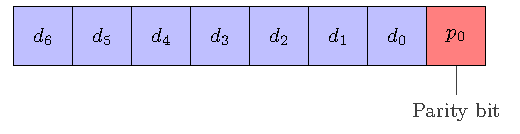
\includegraphics[width=.5\textwidth, page=1]{src/4_strategies/img/simple_parity.pdf}
            \caption{Simple parity codeword}
            \label{fig:simple_parity_codeword}
        \end{figure}
    \end{frame}

    \begin{frame}{Implementation - Simple Parity}
        \begin{figure}
            \centering
            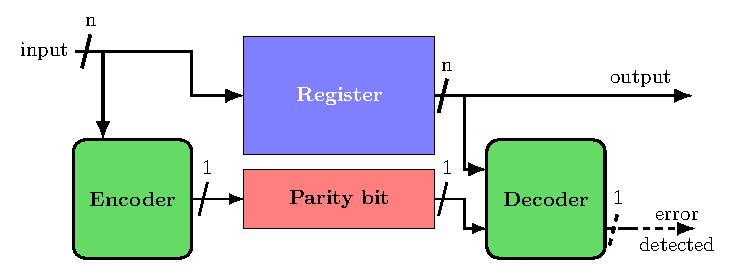
\includegraphics[width=\textwidth, page=1]{src/4_strategies/img/archi_contremesures.pdf}
            \caption{Simple Parity implementation}
            \label{fig:simple_parity_implem}
        \end{figure}
    \end{frame}
%%%%%%%%%%%%%%%%%%%%%%%%%%%%%%%%%%%%%%%%%%%%%%%%%%%%%%%%%%%%%%%%%%%%%%%%%%%%%%%%%%%%%%%%%%%%%%%%%%%%%%%%%%%%
\subsection{Hamming Code}
    \begin{frame}{Detection and correction of single-bit errors - Hamming Code}
        \begin{block}{}
            \begin{itemize}
                \justifying
                \item Linear error-correcting codes invented by Richard W. Hamming~\cite{H-50-bstj}.
                \item Mostly used in digital communication and data storage systems.
                \item Detect and correct single-bit error.
                \item Redundancy bits are placed in power of 2 positions.
                \item The number of redundancy bits depends on the number of bits to be protected {\scriptsize ($ 2^r \ge m + r + 1 $)}
            \end{itemize}
        \end{block}

        \begin{minipage}[c]{0.4\linewidth}
            \begin{equation} \label{equat:hamming_encoder}
                \begin{split}
                    r_{0} &= d_{0} \oplus d_{1} \oplus d_{3} \oplus d_{4} \oplus d_{6} \\
                    r_{1} &= d_{0} \oplus d_{2} \oplus d_{3} \oplus d_{5} \oplus d_{6} \\
                    r_{2} &= d_{1} \oplus d_{2} \oplus d_{3} \\
                    r_{3} &= d_{4} \oplus d_{5} \oplus d_{6}
                \end{split}
            \end{equation}
        \end{minipage}\hfill%
        \begin{minipage}[c]{0.55\linewidth}
            \begin{figure}
                \centering
                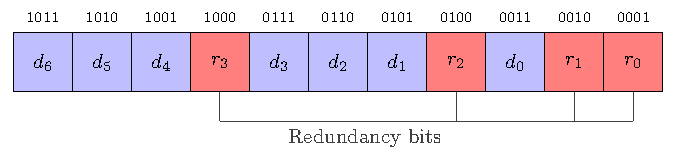
\includegraphics[width=\textwidth, page=1]{src/4_strategies/img/hamming_bit.pdf}
                \caption{Hamming codeword}
                \label{fig:hamming_codeword}
            \end{figure}
        \end{minipage}
    \end{frame}
    
    % \begin{frame}{Implementation - Hamming Code}
    %     \begin{figure}
    %         \centering
    %         \includegraphics[width=.9\textwidth, page=2]{src/4_strategies/img/archi_contremesures.pdf}
    %         \caption{Hamming Code implementation for independant registers}
    %         \label{fig:hamming_code_implem_independant_register}
    %     \end{figure}
    % \end{frame}
    
    % \begin{frame}{Implementation - Hamming Code}
    %     \begin{figure}
    %         \centering
    %         \includegraphics[width=.9\textwidth, page=3]{src/4_strategies/img/archi_contremesures.pdf}
    %         \caption{Hamming Code implementation for Register File}
    %         \label{fig:hamming_code_implem_rf}
    %     \end{figure}
    % \end{frame}
%%%%%%%%%%%%%%%%%%%%%%%%%%%%%%%%%%%%%%%%%%%%%%%%%%%%%%%%%%%%%%%%%%%%%%%%%%%%%%%%%%%%%%%%%%%%%%%%%%%%%%%%%%%%
\subsection{Hamming Code - SECDED}
\begin{frame}{Detection of two-bit errors and correction of single-bit errors - SECDED}
    \begin{block}{}
        \begin{itemize}
            \justifying
            \item Based on Hamming Code.
            \item Detect two-bit error and correct single-bit error.
            \item An additional bit is added: general parity bit
        \end{itemize}
    \end{block}

    \begin{minipage}[c]{0.4\linewidth}
        \begin{equation} \label{equat:secded_encoder}
            \begin{split}
                r_{0}  &= d_{0} \oplus d_{1} \oplus d_{3} \oplus d_{4} \oplus d_{6} \\
                r_{1}  &= d_{0} \oplus d_{2} \oplus d_{3} \oplus d_{5} \oplus d_{6} \\
                r_{2}  &= d_{1} \oplus d_{2} \oplus d_{3} \\
                r_{3}  &= d_{4} \oplus d_{5} \oplus d_{6} \\
                gp_{0} &= \bigoplus_{i=0}^{6} d_{i} \oplus \bigoplus_{j=0}^{3} r_{j}
            \end{split}
        \end{equation}
    \end{minipage}\hfill%
    \begin{minipage}[c]{0.6\linewidth}
        \begin{figure}
            \centering
            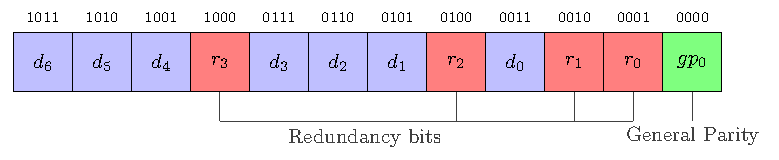
\includegraphics[width=\textwidth, page=1]{src/4_strategies/img/secded.pdf}
            \caption{SECDED codeword}
            \label{fig:secded_codeword}
        \end{figure}
    \end{minipage}
\end{frame}
    
\begin{frame}{Implementation - SECDED}
    \begin{figure}
        \centering
        \includegraphics[width=.8\textwidth, page=4]{src/4_strategies/img/archi_contremesures.pdf}
        \caption{SECDED implementation for independant registers}
        \label{fig:secded_implem_independant_register}
    \end{figure}
\end{frame}

\begin{frame}{Implementation - SECDED}
    \begin{figure}
        \centering
        \includegraphics[width=.9\textwidth, page=5]{src/4_strategies/img/archi_contremesures.pdf}
        \caption{SECDED implementation for Register File}
        \label{fig:secded_implem_rf}
    \end{figure}
\end{frame}
%%%%%%%%%%%%%%%%%%%%%%%%%%%%%%%%%%%%%%%%%%%%%%%%%%%%%%%%%%%%%%%%%%%%%%%%%%%%%%%%%%%%%%%%%%%%%%%%%%%%%%%%%%%%
\begin{frame}{Threat model}
    \begin{block}{Threat model}
        \begin{itemize}
            \item DIFT-related registers + protection-related registers
            \item Single bit-flip in one register
            \item Single bit-flip in two registers at two distinct clock cycles
            \item Single bit-flip in two registers at a given clock cycle
            \item Multi-bit faults in one register at a given clock cycle
            \item Multi-bit faults in two registers at a given clock cycle
        \end{itemize}
    \end{block}
\end{frame}
%%%%%%%%%%%%%%%%%%%%%%%%%%%%%%%%%%%%%%%%%%%%%%%%%%%%%%%%%%%%%%%%%%%%%%%%%%%%%%%%%%%%%%%%%%%%%%%%%%%%%%%%%%%%
\begin{frame}{Implemented strategies - Group composition}
    \begin{table}[t]
        \centering
        \small
        \caption{Grouping composition of implemented strategies}
        \label{tab:strategies_group}
        \begin{tabular}{@{}cccc@{}}
            \toprule
                                & \tableTwoLines{Grouping}{strategy}       & \tableTwoLines{Number of}{groups} & \tableTwoLines{Number of}{registers} \\ \midrule
            Baseline -- D-RI5CY & --                                          & --                                & 55                                   \\
            Strategy 1          & Minimisation of groups                      & 5                                 & 65                                   \\
            Strategy 2          & Protection per pipeline stage               & 7                                 & 69                                   \\
            Strategy 3          & Protection per register                     & 24                                & 103                                  \\
            Strategy 4          & Protection per register with slicing of CSR & 38                                & 131                                  \\
            Strategy 5          & Coupling sliced registers                   & 39                                & 133                                  \\
            \bottomrule
        \end{tabular}
    \end{table}
\end{frame}
%%%%%%%%%%%%%%%%%%%%%%%%%%%%%%%%%%%%%%%%%%%%%%%%%%%%%%%%%%%%%%%%%%%%%%%%%%%%%%%%%%%%%%%%%%%%%%%%%%%%%%%%%%%%
\begin{frame}{Implemented strategies - details}
    \begin{table}[t]
        \centering
        \small
        \caption{Summary of DIFT-related protected registers -- taking SECDED}
        \label{tab:detail_strategies_group}
        \begin{tabular}{@{}cccccc@{}}
            \toprule
                       & \begin{tabular}[c]{@{}c@{}}Number of\\ protected bits\end{tabular} & \begin{tabular}[c]{@{}c@{}}Number of\\ redundancy bits\end{tabular} & \begin{tabular}[c]{@{}c@{}}Number of\\ parity bits\end{tabular} & \begin{tabular}[c]{@{}c@{}}Number of\\ bits\end{tabular} \\ \midrule
            Strategy 1 & 107                                                                & 25                                                                  & 5                                                               & 157                                                      \\
            Strategy 2 & 107                                                                & 30                                                                  & 7                                                               & 164                                                      \\
            Strategy 3 & 107                                                                & 64                                                                  & 24                                                              & 215                                                      \\
            Strategy 4 & 103                                                                & 101                                                                 & 38                                                              & 266                                                      \\
            Strategy 5 & 102                                                                & 114                                                                 & 39                                                              & 280                                                      \\
            \bottomrule
        \end{tabular}
    \end{table}
\end{frame}
%%%%%%%%%%%%%%%%%%%%%%%%%%%%%%%%%%%%%%%%%%%%%%%%%%%%%%%%%%%%%%%%%%%%%%%%%%%%%%%%%%%%%%%%%%%%%%%%%%%%%%%%%%%%